% !TeX root=main.tex
\begin{frame}[fragile]
  \frametitle{AlphaZero}
  \framesubtitle{Base Architecture}

  \begin{center}
    \vcenteredhbox{\begin{tikzpicture}
      \node[circle,
        text=white,
        minimum width=0.3\textwidth,
        path picture={
          \node at (path picture bounding box.center){
            \includegraphics[width=0.3\textwidth]{images/deepmind-logo.jpg}
          };
        }]{};
        \node at (0,0) {\textcolor{black}{\Large\bfseries AlphaZero}};
    \end{tikzpicture}
    }
    \vcenteredhbox{%
      \huge$\,{=}\mkern5mu{}$%
      \raisebox{-0.1em}{%
        $\mathop{\text{PUCT}}
        \limits_{\vphantom{\text{ph}}}^\text{\small a variant of}$
      }%
      $ \mkern1mu{+}\mkern5mu {}$%
      \raisebox{-0.1em}{%
        $\mathop{\text{ResNet}}\limits^\text{\small convolutional}$%
      }%
    }
  \end{center}
\end{frame}

\begin{frame}[fragile]
  \frametitle{Monte--Carlo Tree Search}
  \framesubtitle{An Efficient Way to Achieve Higher Reward}

  \begin{center}
    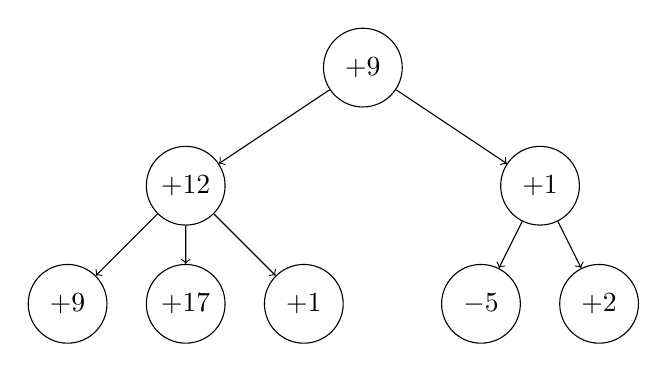
\begin{tikzpicture}[nodes={draw, circle}, ->, minimum size=1cm]
    \node{$+9$}
    child { node {$+12$}
      child { node {$+9$} }
      child { node {$+17$} }
      child { node {$+1$} } }
    child [missing]
    child [missing]
    child { node {$+1$}
      child { node {$-5$} }
      child { node {$+2$} } };
  \end{tikzpicture}
  
  \vspace{2em}
  {\Large $\displaystyle \pi(a|s) \propto N(s, a)^{1/\tau} $}

  \vspace{-1.5em}
  \begin{align*}
    &\text{$\pi$: resulting probability distribution after the search,}\\
    &\text{$N(s, a)$: the $\#$ of visits to $a$ at $s$,\quad $\tau$: temperature constant}
  \end{align*}
\end{center}
\end{frame}

\begin{frame}[fragile]
  \frametitle{PUCT}
  \framesubtitle{Polynomial Upper Confidence bounds applied to Trees}

  \begin{center}
  \vcenteredhbox{$\shortstack{\huge Exploitation\\\normalsize of nodes with high rewards}$}
  \vcenteredhbox{\quad vs.\quad}
  \vcenteredhbox{$\shortstack{\huge Exploration\\\normalsize of new nodes}$}
\end{center}
\end{frame}

\begin{frame}[fragile]
  \frametitle{PUCT}
  \framesubtitle{Polynomial Upper Confidence bounds applied to Trees}

  \begin{center}
  {\large $\displaystyle a_t = \mathop{\operatorname{arg\,max}}\limits_{a\text{: action}} \left[ Q(s_t, a) + c_{\text{puct}} P(a|s_t) \, \frac{\sqrt{\sum_{b} N(s_t, b)}}{1 + N(s_t, a)} \right] $}

  \begin{align*}
    &\text{$s_t$: $t^\text{th}$ state,}\\
    &\text{$a_t$: action to choose at $t^\text{th}$ step,}\\
    &\text{$P(a|s_t)$: prior probability.}
  \end{align*}
\end{center}
\end{frame}

\begin{frame}[fragile]
  \frametitle{Use of Neural Network}

  AlphaZero gets the \gostopemph{prior probability distribution} and the \gostopemph{expected} \!\gostopemph{value}\,of unvisited nodes from the neural network.

  \vspace{1em}

  \begin{center}
    \Large $\text{NN}\colon \text{nonterminal state}\mapsto (\text{policy}, \text{value}).$
  \end{center}

  \vspace{1em}

  In fact, $P(a|s)$ is the weighted average of the policy from the NN and a Dirichlet random noise.

  \vspace{1em}

  \begin{center}
    \large $P(\cdot|s) = (1-\epsilon)\,\text{NN}_{\text{policy}}(s) + \epsilon E,\quad E\sim \mathop{\mathrm{Dir}(\symbf\alpha)}\limits_{\mathclap{\symbf\alpha = (\alpha,\dots,\alpha)}}.$
  \end{center}
\end{frame}

\begin{frame}[fragile]
  \frametitle{Train the Neural Network}

  The training data is provided by the MCTS simulation.

  \vspace{1em}

  \begin{center}
    \begin{tikzpicture}[-{>[length=.5em,width=1em]},node distance=20em,node/.style={circle,draw},minimum size=4em]

    \node[node] (mcts) {MCTS};
    \node[node] (nn) [right of=mcts] {NN};

    \path
    (mcts) edge [bend right] node [yshift=-1em] {training data} (nn)
    (nn) edge [bend right] node [yshift=1em] {policy \& value of unvisited nodes} (mcts);      
    \end{tikzpicture}
  \end{center}
\end{frame}

\begin{frame}[fragile]
  \frametitle{Self-Play}
  \framesubtitle{Evolve by Competing with Itself}

  \hspace*{-1.5em}\begin{tikzpicture}[-{>[length=.5em,width=1em]},node distance=10em,node/.style={circle,draw},minimum size=4em]

  \node[node] (s) {state};
  \node[node] (p0) [right=11em of s] {policy$^*$};
  \node[node] (p) [below of=p0] {policy};
  \node[node] (a) [below of=s] {action};

  \path
  (s) edge node [yshift=1em] {NN} (p0)
  (p0) edge node [right] {(mask illegal actions)} (p)
  (p) edge node [yshift=-1em] {arg\,max$^\text{\dagger}$} (a)
  (a) edge node [left] {$\begin{matrix}\text{play the action}\\[-0.2em]\text{to get a new state}\end{matrix}$} (s);
  \end{tikzpicture}
  
  \vspace{1em}

  \small\dagger: In fact, AlphaZero randomly chose an action from $\text{NN}_\text{policy}(\cdot|s)^{1/\tau}$ for $\tau\approx 0$, but it is not that different from the arg\,max.
\end{frame}
